%!TEX program = xelatex

\documentclass{ctexart}
    \usepackage{amsmath}
    \usepackage{pgf}
    \usepackage{tikz}
    \usetikzlibrary{arrows,automata}
    % \usepackage[latin1]{inputenc}
    \usepackage{verbatim}
    \title{Solution for Homework1}
    \author{徐翔哲(161250170)} 
    
\begin{document}
\maketitle
\newpage
\section{Problem1}
\subsection{a}

Firstly, we can get the automata as follows.\\

% 1-1-1
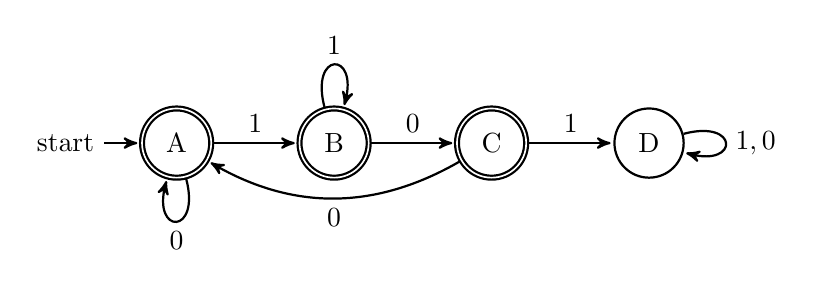
\begin{tikzpicture}
	[->,>=stealth',shorten >=1pt,auto,node distance=2cm,
		thick,base node/.style={circle,draw,minimum size=16pt}, real node/.style={double,circle,draw,minimum size=35pt}]

	\node[initial, initial text={start},accepting, state] (A) {A};
	\node[accepting, state] (B)[right of = A] {B};
	\node[accepting, state] (C)[right of = B] {C};
	\node[state] (D)[right of = C] {D};

	% \node[initial,initial text={}, accepting, state] (1) {$\epsilon$};
	% \node[state](2)[right of=1 ]{$51$}[above];

	\path[]
	(A) edge [loop below]   node {$0$}  (A)
	edge                node {$1$}     (B)
	(B) edge [loop above]   node {$1$}  (B)
	edge                node {$0$}  (C)
	(C) edge [bend left]   node {$0$}  (A)
	edge                node {$1$}  (D)
	(D) edge [loop right]   node {$1,0$} (D)
	;


\end{tikzpicture}

Then we just delete state D since it contributes nothing to the accepted strings.\\

% 1-1-2
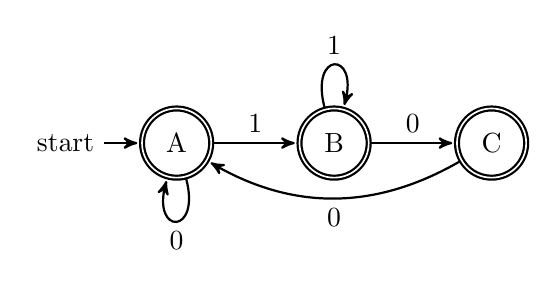
\begin{tikzpicture}
	[->,>=stealth',shorten >=1pt,auto,node distance=2cm,
		thick,base node/.style={circle,draw,minimum size=16pt}, real node/.style={double,circle,draw,minimum size=35pt}]


	\node[initial, initial text={start},accepting, state] (A) {A};
	\node[accepting, state] (B)[right of = A] {B};
	\node[accepting, state] (C)[right of = B] {C};

	\path[]
	(A) edge [loop below]   node {$0$}  (A)
	edge                node {$1$}     (B)
	(B) edge [loop above]   node {$1$}  (B)
	edge                node {$0$}  (C)
	(C) edge [bend left]   node {$0$}  (A)
	;
\end{tikzpicture}

First, we pick A as the accepting state. Then we get $(0^*+11^*00)^*$\\

% branch1-1
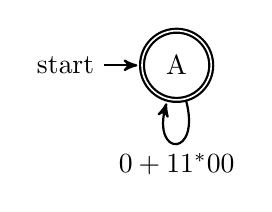
\begin{tikzpicture}
	[->,>=stealth',shorten >=1pt,auto,node distance=2cm,
		thick,base node/.style={circle,draw,minimum size=16pt}, real node/.style={double,circle,draw,minimum size=35pt}]


	\node[initial, initial text={start},accepting, state] (A) {A};

	\path[]
	(A) edge [loop below]   node {$0+11^*00$}  (A)
	% edge                node {$1$}     (B)
	% (B) edge [loop above]   node {$1$}  (B)
	%     edge                node {$0$}  (C)
	% (C) edge [bend left]   node {$0$}  (A)
	;
\end{tikzpicture}

Then we choose state C as the accepting state. Then we get $(0+11^*00)^*11^*0$\\

% branch 1-2
\begin{tikzpicture}
	[->,>=stealth',shorten >=1pt,auto,node distance=2cm,
		thick,base node/.style={circle,draw,minimum size=16pt}, real node/.style={double,circle,draw,minimum size=35pt}]


	\node[initial, initial text={start},accepting, state] (A) {A};
	\node[accepting, state] (C)[right of = B] {C};

	\path[]
	(A) edge [loop below]   node {$0$}  (A)
	edge                node {$11^*0$}     (C)
	(C) edge [bend left]   node {$0$}  (A)
	;
\end{tikzpicture}

Finally, we choose B as the accepting state. Then we get $(0+11^*00)^*11^* $\\
% branch 2
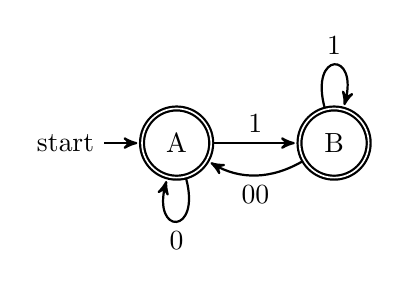
\begin{tikzpicture}
	[->,>=stealth',shorten >=1pt,auto,node distance=2cm,
		thick,base node/.style={circle,draw,minimum size=16pt}, real node/.style={double,circle,draw,minimum size=35pt}]


	\node[initial, initial text={start},accepting, state] (A) {A};
	\node[accepting, state] (B)[right of = A] {B};

	\path[]
	(A) edge [loop below]   node {$0$}  (A)
	edge                node {$1$}     (B)
	(B) edge [loop above]   node {$1$}  (B)
	edge [bend left]    node {$00$}  (A)
	;
\end{tikzpicture}

In all, we have $(0^*+11^*00)^* + (0+11^*00)^*11^*0 + (0+11^*00)^*11^* $

\subsection{b}

First, we get the DFA as follows:\\

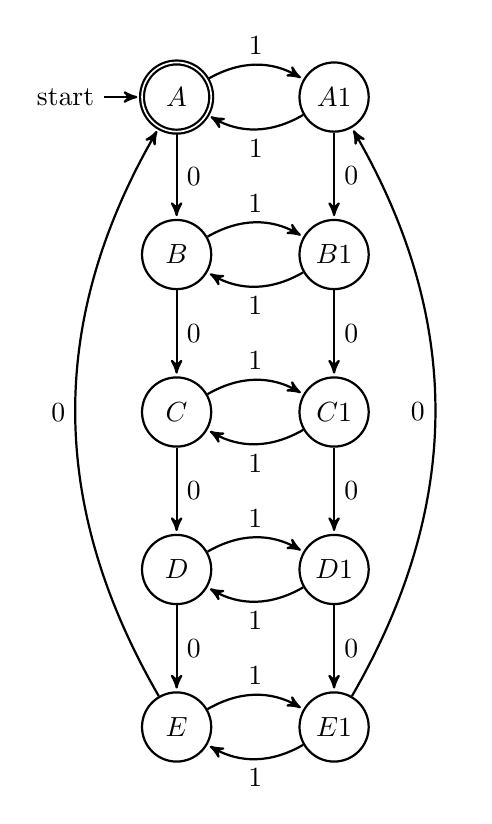
\begin{tikzpicture}
	[->,>=stealth',shorten >=1pt,auto,node distance=2cm,
		thick,base node/.style={circle,draw,minimum size=16pt}, real node/.style={double,circle,draw,minimum size=35pt}]

	\node[initial, initial text={start}, accepting, state] (A) {$A$};
	\node[state]    (A1)    [right of = A]  {$A1$};
	\node[state]    (B)     [below of = A]  {$B$};
	\node[state]    (B1)     [below of = A1]  {$B1$};
	\node[state]    (C)     [below of = B]  {$C$};
	\node[state]    (C1)     [below of = B1]  {$C1$};
	\node[state]    (D)     [below of = C]  {$D$};
	\node[state]    (D1)     [below of = C1]  {$D1$};
	\node[state]    (E)     [below of = D]  {$E$};
	\node[state]    (E1)     [below of = D1]  {$E1$};

	\path[]
	(A) edge [bend left]   node {$1$}  (A1)
	edge    node {$0$}  (B)
	(A1) edge [bend left]  node {$1$}  (A)
	edge    node {$0$}  (B1)
	(B) edge [bend left]   node {$1$}  (B1)
	edge    node {$0$}  (C)

	(B1) edge [bend left]  node {$1$}  (B)
	edge    node {$0$}  (C1)
	(C) edge [bend left]   node {$1$}  (C1)
	edge    node {$0$}  (D)
	(C1) edge [bend left]  node {$1$}  (C)
	edge    node {$0$}  (D1)
	(D) edge [bend left]   node {$1$}  (D1)
	edge    node {$0$}  (E)
	(D1) edge [bend left]  node {$1$}  (D)
	edge    node {$0$}  (E1)
	(E) edge [bend left]   node {$1$}  (E1)
	edge [bend left]   node {$0$}  (A)
	(E1) edge [bend left]  node {$1$}  (E)
	edge [bend right]   node {$0$}  (A1)

	;

\end{tikzpicture}\\

Then we delete state B1.\\


\begin{tikzpicture}
	[->,>=stealth',shorten >=1pt,auto,node distance=2cm,
		thick,base node/.style={circle,draw,minimum size=16pt}, real node/.style={double,circle,draw,minimum size=35pt}]

	\node[initial, initial text={start}, accepting, state] (A) {$A$};
	\node[state]    (A1)    [right of = A]  {$A1$};
	\node[state]    (B)     [below of = A]  {$B$};
	% \node[state]    (B1)     [below of = A1]  {$B1$};
	\node[state]    (C)     [below of = B]  {$C$};
	\node[state]    (C1)     [below of = B1]  {$C1$};
	\node[state]    (D)     [below of = C]  {$D$};
	\node[state]    (D1)     [below of = C1]  {$D1$};
	\node[state]    (E)     [below of = D]  {$E$};
	\node[state]    (E1)     [below of = D1]  {$E1$};

	\path[]
	(A) edge [bend left]   node {$1$}  (A1)
	edge    node {$0$}  (B)
	(A1) edge [bend left]  node {$1$}  (A)
	edge    node {$01$}  (B)
	edge    node {$00$}  (C1)
	(B) edge [loop right]   node {$11$}  (B)
	edge    node {$0$}  (C)
	edge    node {$10$}  (C1)

	% (B1) edge [bend left]  node {$1$}  (B)
	(C) edge [bend left]   node {$1$}  (C1)
	edge    node {$0$}  (D)
	(C1) edge [bend left]  node {$1$}  (C)
	edge    node {$0$}  (D1)
	(D) edge [bend left]   node {$1$}  (D1)
	edge    node {$0$}  (E)
	(D1) edge [bend left]  node {$1$}  (D)
	edge    node {$0$}  (E1)
	(E) edge [bend left]   node {$1$}  (E1)
	edge [bend left]   node {$0$}  (A)
	(E1) edge [bend left]  node {$1$}  (E)
	edge [bend right]   node {$0$}  (A1)

	;

\end{tikzpicture}\\

Then we delete state C.\\

\begin{tikzpicture}
	[->,>=stealth',shorten >=1pt,auto,node distance=2cm,
		thick,base node/.style={circle,draw,minimum size=16pt}, real node/.style={double,circle,draw,minimum size=35pt}]

	\node[initial, initial text={start}, accepting, state] (A) {$A$};
	\node[state]    (A1)    [right of = A]  {$A1$};
	\node[state]    (B)     [below of = A]  {$B$};
	% \node[state]    (B1)     [below of = A1]  {$B1$};
	% \node[state]    (C)     [below of = B]  {$C$};
	\node[state]    (C1)     [below of = B1]  {$C1$};
	\node[state]    (D)     [below of = C]  {$D$};
	\node[state]    (D1)     [below of = C1]  {$D1$};
	\node[state]    (E)     [below of = D]  {$E$};
	\node[state]    (E1)     [below of = D1]  {$E1$};

	\path[]
	(A) edge [bend left]   node {$1$}  (A1)
	edge    node {$0$}  (B)
	(A1) edge [bend left]  node {$1$}  (A)
	edge    node {$01$}  (B)
	edge    node {$00$}  (C1)
	(B) edge [loop right]   node {$11$}  (B)
	% edge    node {$0$}  (C)
	edge [bend right]   node {$10+01$}  (C1)
	edge  [bend right]  node {$00$}  (D)

	% (B1) edge [bend left]  node {$1$}  (B)
	(C1) edge [loop left]   node {$11$}  (C1)
	edge    node {$10$}  (D)
	(C1) edge    node {$0$}  (D1)
	(D) edge [bend left]   node {$1$}  (D1)
	edge    node {$0$}  (E)
	(D1) edge [bend left]  node {$1$}  (D)
	edge    node {$0$}  (E1)
	(E) edge [bend left]   node {$1$}  (E1)
	edge [bend left]   node {$0$}  (A)
	(E1) edge [bend left]  node {$1$}  (E)
	edge [bend right]   node {$0$}  (A1)

	;

\end{tikzpicture}\\

Then we delete state D1.\\

\begin{tikzpicture}
	[->,>=stealth',shorten >=1pt,auto,node distance=2cm,
		thick,base node/.style={circle,draw,minimum size=16pt}, real node/.style={double,circle,draw,minimum size=35pt}]

	\node[initial, initial text={start}, accepting, state] (A) {$A$};
	\node[state]    (A1)    [right of = A]  {$A1$};
	\node[state]    (B)     [below of = A]  {$B$};
	% \node[state]    (B1)     [below of = A1]  {$B1$};
	% \node[state]    (C)     [below of = B]  {$C$};
	\node[state]    (C1)     [below of = B1]  {$C1$};
	\node[state]    (D)     [below of = C]  {$D$};
	% \node[state]    (D1)     [below of = C1]  {$D1$};
	\node[state]    (E)     [below of = D]  {$E$};
	\node[state]    (E1)     [below of = D1]  {$E1$};

	\path[]
	(A) edge [bend left]   node {$1$}  (A1)
	edge    node {$0$}  (B)
	(A1) edge [bend left]  node {$1$}  (A)
	edge    node {$01$}  (B)
	edge    node {$00$}  (C1)
	(B) edge [loop right]   node {$11$}  (B)
	% edge    node {$0$}  (C)
	edge [bend right]   node {$10+01$}  (C1)
	edge  [bend right]  node {$00$}  (D)

	% (B1) edge [bend left]  node {$1$}  (B)
	(C1) edge [loop left]   node {$11$}  (C1)
	edge    node {$10+01$}  (D)
	edge    node {$00$}  (E1)
	% (C1) edge    node {$0$}  (D1)
	(D) edge [loop right]   node {$11$}  (D)
	edge    node {$10$}  (E1)
	edge    node {$0$}  (E)
	% (D1) edge [bend left]  node {$1$}  (D)
	% edge    node {$0$}  (E1)
	(E) edge [bend left]   node {$1$}  (E1)
	edge [bend left]   node {$0$}  (A)
	(E1) edge [bend left]  node {$1$}  (E)
	edge [bend right]   node {$0$}  (A1)

	;

\end{tikzpicture}\\

Then we delete state E.\\


\begin{tikzpicture}
	[->,>=stealth',shorten >=1pt,auto,node distance=2cm,
		thick,base node/.style={circle,draw,minimum size=16pt}, real node/.style={double,circle,draw,minimum size=35pt}]

	\node[initial, initial text={start}, accepting, state] (A) {$A$};
	\node[state]    (A1)    [right of = A]  {$A1$};
	\node[state]    (B)     [below of = A]  {$B$};
	% \node[state]    (B1)     [below of = A1]  {$B1$};
	% \node[state]    (C)     [below of = B]  {$C$};
	\node[state]    (C1)     [below of = B1]  {$C1$};
	\node[state]    (D)     [below of = C]  {$D$};
	% \node[state]    (D1)     [below of = C1]  {$D1$};
	% \node[state]    (E)     [below of = D]  {$E$};
	\node[state]    (E1)     [below of = D1]  {$E1$};

	\path[]
	(A) edge [bend left]   node {$1$}  (A1)
	edge    node {$0$}  (B)
	(A1) edge [bend left]  node {$1$}  (A)
	edge    node {$01$}  (B)
	edge    node {$00$}  (C1)
	(B) edge [loop right]   node {$11$}  (B)
	% edge    node {$0$}  (C)
	edge [bend right]   node {$10+01$}  (C1)
	edge  [bend right]  node {$00$}  (D)

	% (B1) edge [bend left]  node {$1$}  (B)
	(C1) edge [loop left]   node {$11$}  (C1)
	edge    node {$10+01$}  (D)
	edge    node {$00$}  (E1)
	% (C1) edge    node {$0$}  (D1)
	(D) edge [loop right]   node {$11$}  (D)
	edge    node {$10+01$}  (E1)
	edge [bend left]   node {$00$}  (A)

	% edge    node {$0$}  (E)
	% (D1) edge [bend left]  node {$1$}  (D)
	% edge    node {$0$}  (E1)
	% (E) edge [bend left]   node {$1$}  (E1)
	% edge [bend left]   node {$0$}  (A)
	(E1) edge [loop left]  node {$11$}  (E1)
	edge [bend left]   node {$10$}  (A)

	edge [bend right]   node {$0$}  (A1)

	;

\end{tikzpicture}\\

Then we delete state B where $L_1=10+01$.\\

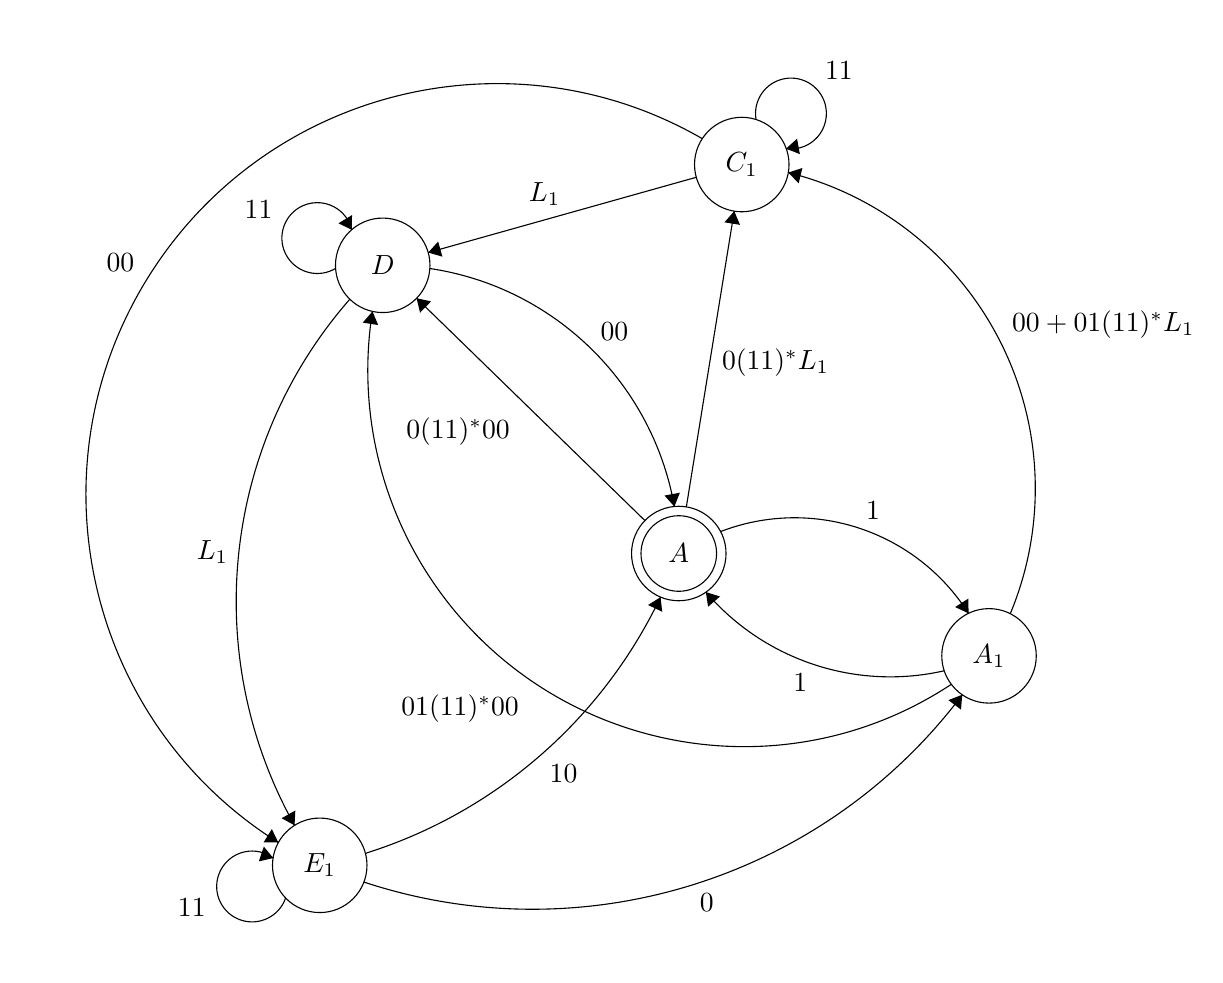
\begin{tikzpicture}[scale=0.2]
	\tikzstyle{every node}+=[inner sep=0pt]
	\draw [black] (41,-32.8) circle (3);
	\draw (41,-32.8) node {$A$};
	\draw [black] (41,-32.8) circle (2.4);
	\draw [black] (60.7,-39.3) circle (3);
	\draw (60.7,-39.3) node {$A_1$};
	\draw [black] (18.2,-52.6) circle (3);
	\draw (18.2,-52.6) node {$E_1$};
	\draw [black] (45,-8.1) circle (3);
	\draw (45,-8.1) node {$C_1$};
	\draw [black] (22.2,-14.5) circle (3);
	\draw (22.2,-14.5) node {$D$};
	\draw [black] (43.65,-31.409) arc (111.12351:32.35595:13.067);
	\fill [black] (59.4,-36.6) -- (59.39,-35.66) -- (58.55,-36.2);
	\draw (53.34,-30.65) node [above] {$1$};
	\draw [black] (45.908,-5.253) arc (190.05134:-97.94866:2.25);
	\draw (51.17,-2.76) node [above] {$11$};
	\fill [black] (47.81,-7.09) -- (48.69,-7.44) -- (48.51,-6.46);
	\draw [black] (19.218,-14.69) arc (301.38014:13.38014:2.25);
	\draw (15.23,-10.98) node [left] {$11$};
	\fill [black] (20.24,-12.25) -- (20.25,-11.31) -- (19.39,-11.83);
	\draw [black] (16.037,-54.662) arc (-18.64598:-306.64598:2.25);
	\draw (10.99,-55.26) node [left] {$11$};
	\fill [black] (15.25,-52.14) -- (14.65,-51.41) -- (14.33,-52.35);
	\draw [black] (47.954,-8.611) arc (76.02951:-22.60596:20.677);
	\fill [black] (47.95,-8.61) -- (48.61,-9.29) -- (48.85,-8.32);
	\draw (62.13,-18.27) node [right] {$00+01(11)^*L_1$};
	\draw [black] (41.48,-29.84) -- (44.52,-11.06);
	\fill [black] (44.52,-11.06) -- (43.9,-11.77) -- (44.89,-11.93);
	\draw (43.71,-20.67) node [right] {$0(11)^*L_1$};
	\draw [black] (58.307,-41.106) arc (-56.55381:-189.02189:23.89);
	\fill [black] (21.55,-17.43) -- (20.93,-18.14) -- (21.91,-18.29);
	\draw (27.11,-41.76) node [below] {$01(11)^*00$};
	\draw [black] (57.858,-40.246) arc (-77.1518:-139.36873:15.426);
	\fill [black] (42.72,-35.25) -- (42.86,-36.18) -- (43.62,-35.53);
	\draw (48.71,-40.39) node [below] {$1$};
	\draw [black] (25.19,-14.701) arc (81.51747:10.0268:18.548);
	\fill [black] (40.72,-29.82) -- (41.07,-28.94) -- (40.09,-29.12);
	\draw (36.91,-19.28) node [above] {$00$};
	\draw [black] (38.85,-30.71) -- (24.35,-16.59);
	\fill [black] (24.35,-16.59) -- (24.57,-17.51) -- (25.27,-16.79);
	\draw (26.98,-24.13) node [below] {$0(11)^*00$};
	\draw [black] (59.004,-41.773) arc (-36.96172:-108.28418:34.149);
	\fill [black] (59,-41.77) -- (58.12,-42.11) -- (58.92,-42.71);
	\draw (42.78,-54.37) node [below] {$0$};
	\draw [black] (42.11,-8.91) -- (25.09,-13.69);
	\fill [black] (25.09,-13.69) -- (25.99,-13.95) -- (25.72,-12.99);
	\draw (32.48,-10.72) node [above] {$L_1$};
	\draw [black] (15.573,-51.154) arc (-122.12951:-299.98716:26.094);
	\fill [black] (15.57,-51.15) -- (15.16,-50.3) -- (14.63,-51.15);
	\draw (6.46,-14.33) node [left] {$00$};
	\draw [black] (39.842,-35.566) arc (-25.49039:-72.56614:31.076);
	\fill [black] (39.84,-35.57) -- (39.05,-36.07) -- (39.95,-36.5);
	\draw (33.68,-46.15) node [below] {$10$};
	\draw [black] (16.603,-50.062) arc (-150.77208:-221.21462:29.125);
	\fill [black] (16.6,-50.06) -- (16.65,-49.12) -- (15.78,-49.61);
	\draw (12.41,-32.7) node [left] {$L_1$};
\end{tikzpicture}\\


Then we delete E1.\\

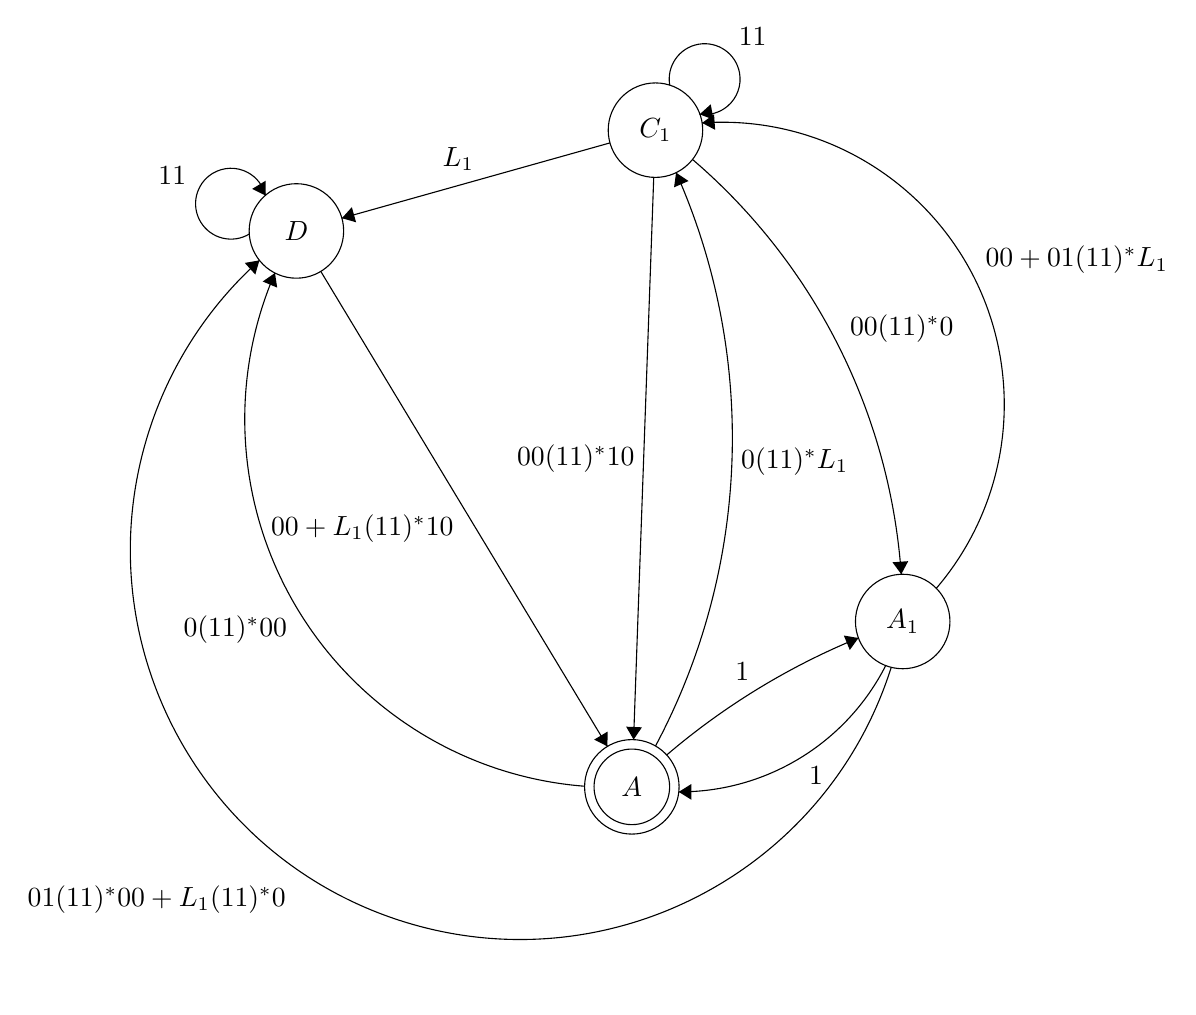
\begin{tikzpicture}[scale=0.2]
	\tikzstyle{every node}+=[inner sep=0pt]
	\draw [black] (43.5,-49.8) circle (3);
	\draw (43.5,-49.8) node {$A$};
	\draw [black] (43.5,-49.8) circle (2.4);
	\draw [black] (60.7,-39.3) circle (3);
	\draw (60.7,-39.3) node {$A_1$};
	\draw [black] (45,-8.1) circle (3);
	\draw (45,-8.1) node {$C_1$};
	\draw [black] (22.2,-14.5) circle (3);
	\draw (22.2,-14.5) node {$D$};
	\draw [black] (45.714,-47.777) arc (130.50667:112.29855:45.072);
	\fill [black] (57.89,-40.35) -- (56.96,-40.19) -- (57.34,-41.11);
	\draw (50.51,-43.08) node [above] {$1$};
	\draw [black] (45.908,-5.253) arc (190.05134:-97.94866:2.25);
	\draw (51.17,-2.76) node [above] {$11$};
	\fill [black] (47.81,-7.09) -- (48.69,-7.44) -- (48.51,-6.46);
	\draw [black] (19.218,-14.69) arc (301.38014:13.38014:2.25);
	\draw (15.23,-10.98) node [left] {$11$};
	\fill [black] (20.24,-12.25) -- (20.25,-11.31) -- (19.39,-11.83);
	\draw [black] (47.961,-7.641) arc (94.0212:-40.59765:17.931);
	\fill [black] (47.96,-7.64) -- (48.79,-8.08) -- (48.72,-7.09);
	\draw (65.93,-16.35) node [right] {$00+01(11)^*L_1$};
	\draw [black] (46.314,-10.796) arc (23.91032:-28.03054:41.598);
	\fill [black] (46.31,-10.8) -- (46.18,-11.73) -- (47.1,-11.33);
	\draw (50.41,-29.16) node [right] {$0(11)^*L_1$};
	\draw [black] (59.972,-42.208) arc (-17.53501:-228.04068:24.732);
	\fill [black] (19.85,-16.37) -- (18.92,-16.53) -- (19.59,-17.27);
	\draw (13.33,-56.05) node [below] {$01(11)^*00+L_1(11)^*0$};
	\draw [black] (59.623,-42.094) arc (-26.93721:-90.25757:14.671);
	\fill [black] (46.48,-50.12) -- (47.28,-50.62) -- (47.28,-49.62);
	\draw (55.19,-48.47) node [below] {$1$};
	\draw [black] (23.75,-17.07) -- (41.95,-47.23);
	\fill [black] (41.95,-47.23) -- (41.96,-46.29) -- (41.11,-46.8);
	\draw (32.21,-33.42) node [left] {$00+L_1(11)^*10$};
	\draw [black] (40.502,-49.761) arc (-94.41412:-203.37236:23.384);
	\fill [black] (20.84,-17.17) -- (20.06,-17.71) -- (20.98,-18.1);
	\draw (21.64,-39.79) node [left] {$0(11)^*00$};
	\draw [black] (42.11,-8.91) -- (25.09,-13.69);
	\fill [black] (25.09,-13.69) -- (25.99,-13.95) -- (25.72,-12.99);
	\draw (32.48,-10.72) node [above] {$L_1$};
	\draw [black] (44.89,-11.1) -- (43.61,-46.8);
	\fill [black] (43.61,-46.8) -- (44.14,-46.02) -- (43.14,-45.98);
	\draw (43.7,-28.94) node [left] {$00(11)^*10$};
	\draw [black] (47.353,-9.96) arc (49.41298:4.01057:38.205);
	\fill [black] (60.61,-36.3) -- (61.05,-35.47) -- (60.05,-35.54);
	\draw (57.32,-20.69) node [right] {$00(11)^*0$};
\end{tikzpicture}\\

Then we can delete state C1. And
$$
	L_1=10+01
$$
$$
	L_2=00+01(11)^*L_1\\
$$
$$
	L_3=00(11)^*10\\
$$\\


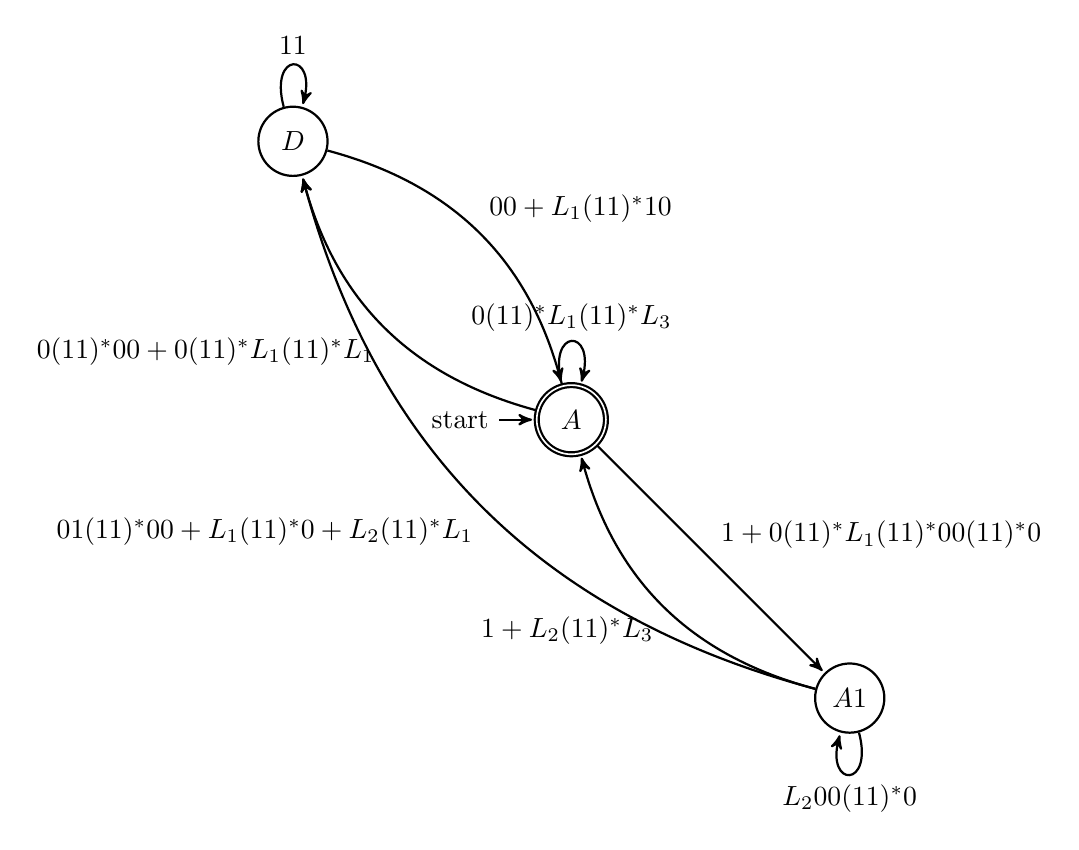
\begin{tikzpicture}
	[->,>=stealth',shorten >=1pt,auto,node distance=5cm,
		thick,base node/.style={circle,draw,minimum size=16pt}, real node/.style={double,circle,draw,minimum size=35pt}]

	\node[initial, initial text={start}, accepting, state] (A) {$A$};
	\node[state]    (A1)    [below right of = A]  {$A1$};
	% \node[state]    (B)     [below of = A]  {$B$};
	% \node[state]    (B1)     [below of = A1]  {$B1$};
	% \node[state]    (C)     [below of = B]  {$C$};
	% \node[state]    (C1)     [below of = B1]  {$C1$};
	\node[state]    (D)     [above left of = A]  {$D$};
	% \node[state]    (D1)     [below of = C1]  {$D1$};
	% \node[state]    (E)     [below of = D]  {$E$};
	% \node[state]    (E1)     [below of = D1]  {$E1$};

	\path[]
	(A) edge    node {$1+0(11)^*L_1(11)^*00(11)^*0$}  (A1)
	(A) edge [loop above]   node {$0(11)^*L_1(11)^*L_3$}  (A)
	(A1) edge [bend left]   node {$1+L_2(11)^*L_3$}  (A)
	(A1) edge [loop below]   node {$L_200(11)^*0 $}  (A1)
	(A1) edge [bend left]   node {$01(11)^*00+L_1(11)^*0+L_2(11)^*L_1 $}  (D)
	(D) edge [loop above]   node {$11$}  (D)
	(D) edge [bend left]   node {$00+L_1(11)^*10$}  (A)
	(A) edge [bend left]   node {$0(11)^*00+0(11)^*L_1(11)^*L_1 $}  (D)


	;

\end{tikzpicture}\\

Finally,
\[R=0(11)^*L_1(11)^*L_3+L_5(11)^*(00+L_1(11)^*10) \]
\[S=1+L_2(11)^*L_3+L_4(11)^*(00+L_1(11)^*10) \]
\[T=L_200(11)^*0 \]
\[L_1=10+01 \]
\[L_2=00+01(11)^*L_1 \]
\[L_3=00(11)^*10 \]
\[L_4=01(11)^*00+L_1(11)^*0+L_2(11)^*L_1 \]
\[L_5=0(11)^*00+0(11)^*L_1(11)^*L_1 \]
\[L_6=1+0(11)^*L_1(11)^*00(11)^*0 \]

And the answer should be $(R+L_6T^*S)^*$.\\

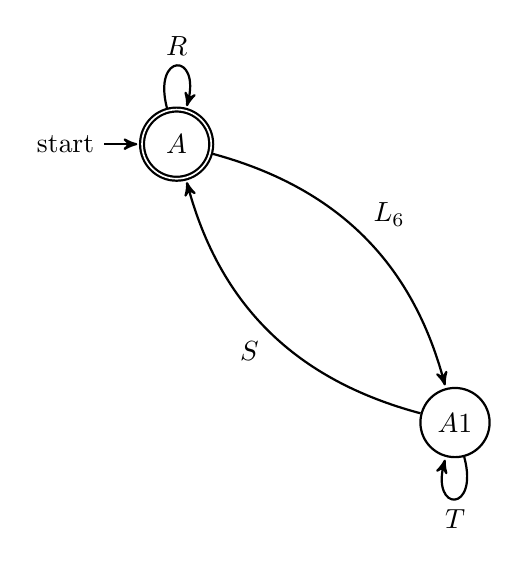
\begin{tikzpicture}
	[->,>=stealth',shorten >=1pt,auto,node distance=5cm,
		thick,base node/.style={circle,draw,minimum size=16pt}, real node/.style={double,circle,draw,minimum size=35pt}]

	\node[initial, initial text={start}, accepting, state] (A) {$A$};
	\node[state]    (A1)    [below right of = A]  {$A1$};
	% \node[state]    (B)     [below of = A]  {$B$};
	% \node[state]    (B1)     [below of = A1]  {$B1$};
	% \node[state]    (C)     [below of = B]  {$C$};
	% \node[state]    (C1)     [below of = B1]  {$C1$};
	% \node[state]    (D)     [above left of = A]  {$D$};
	% \node[state]    (D1)     [below of = C1]  {$D1$};
	% \node[state]    (E)     [below of = D]  {$E$};
	% \node[state]    (E1)     [below of = D1]  {$E1$};

	\path[]
	(A) edge [loop above]   node {$R$}  (A)
	(A) edge [bend left]   node {$L_6$}  (A1)
	(A1) edge [bend left]   node {$S$}  (A)
	(A1) edge [loop below]   node {$T $}  (A1)
	;

\end{tikzpicture}\\



\end{document}